\documentclass{article}
\usepackage{amsmath}
\usepackage{graphicx}
\usepackage{wrapfig}
\usepackage{verbatim}
\usepackage{spverbatim}
\title{SPQR 0.9.7\\A simulation package for the prediction, refinement and simulation of RNA structures.}
\author{Sim\'on Poblete}
\date{}
\begin{document}
\maketitle
\section{Introduction.}

SPQR (SPlit and conQueR) is a coarse-grained representation of RNA \cite{spqr1, spqr2}, which is implemented in the present software. The energy function can be used to score structures, predict three-dimensional structures from a given sequence, explore the conformational space and optimize structures as well. 



\section{Features.}




As a coarse-grained model, SPQR is defined by its degrees of freedom and its energy function. As shown in Figure \ref{cg-rep}, each nucleoside is represented by an anisotropic particle, while the phosphate group is a point particle.

Thus, the base is an anisotropic object with a virtual site which stands for the sugar group.
This representation allows the introduction of directional interactions and the possibility of forming stacking, canonical and non-canonical base-pairs and base-phosphate interactions. In addition, through the interactions between a nucleoside and its topologically connected phosphate groups, it can specify the state of the glycosidic bond angle and sugar pucker. The relative weight of the interactions considers the number of hydrogen bonds present in the base-pairs while it has been adjusted by fitting a set of x-ray structures for the rest of interactions.

%\begin{wrapfigure}{r}{0.25\textwidth}
\begin{figure}
\begin{center}
  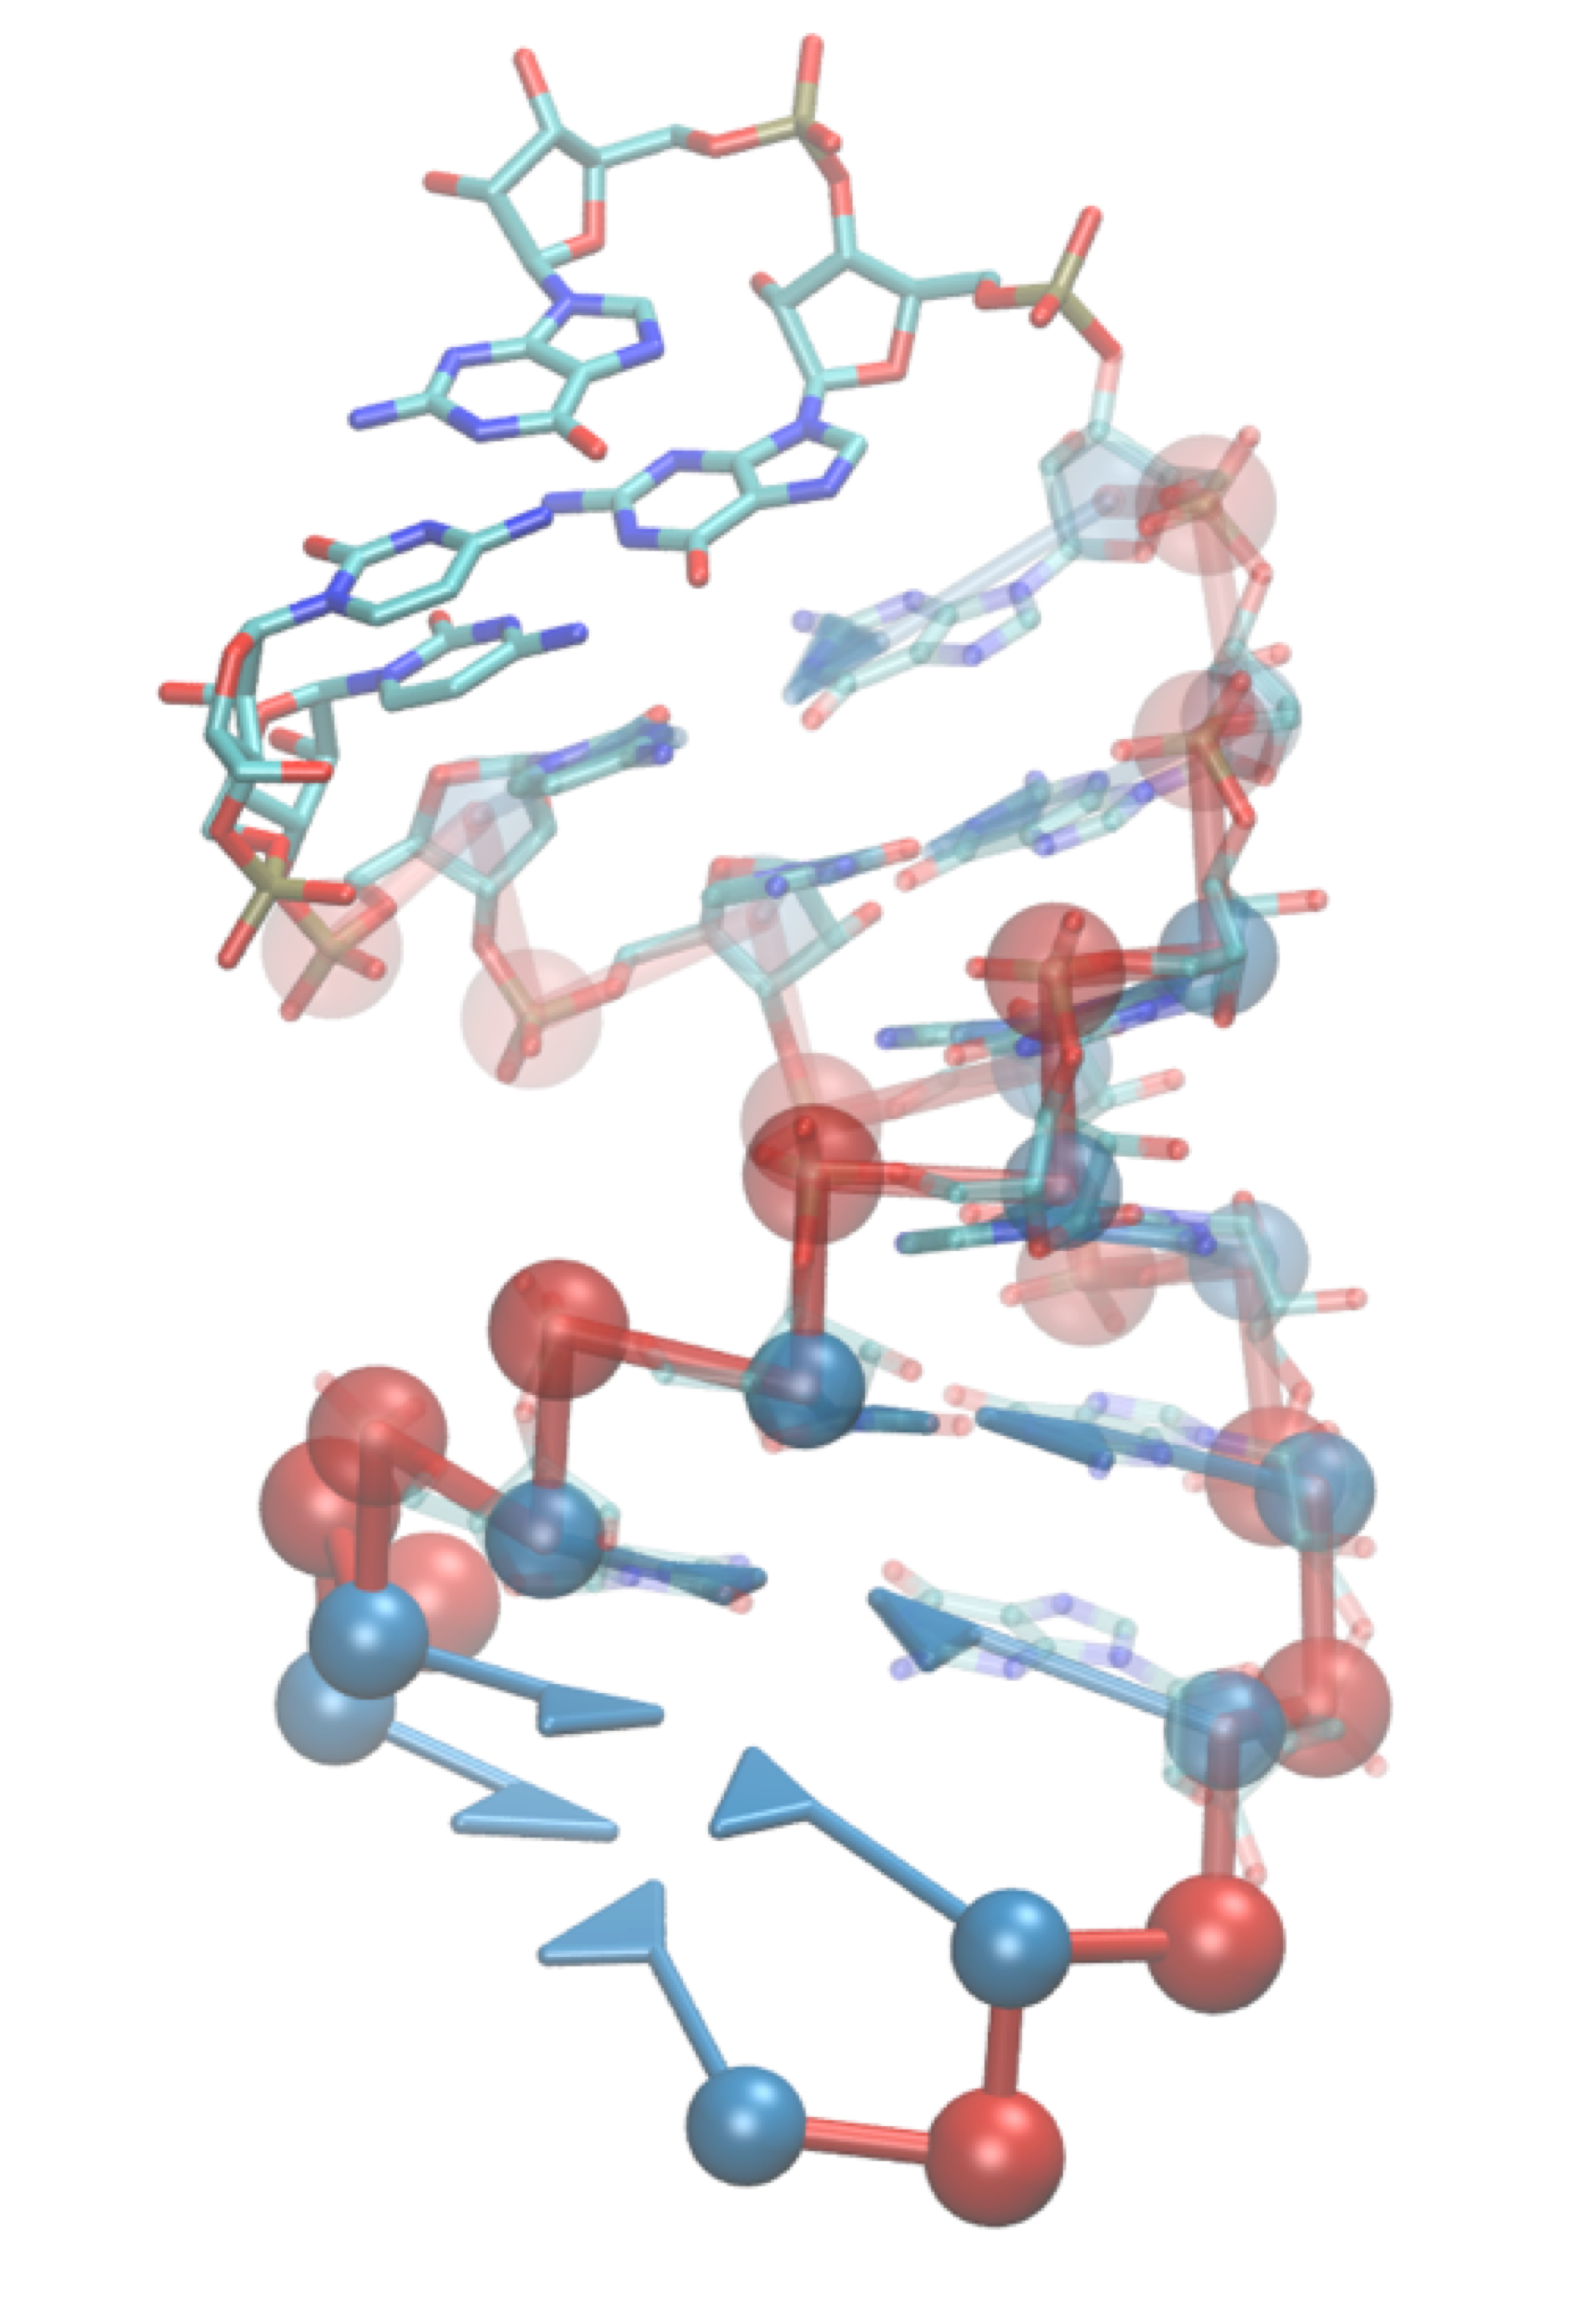
\includegraphics[width=5cm]{src/rnacg.png}
  \caption{SPQR representation of a RNA duplex.}
\label{cg-rep}
\end{center}
\end{figure}
%\end{wrapfigure}


\section{Compiling and installing.}

To compile, one has to run the \verb ./configure ~ script in the \verb src/ directory, which can be generated using  \verb autoconf . Once this is ready, just compile using  \verb make ~  and \verb make ~ \verb install ~  to create the binary files (in the \verb bin ~  directory) and the tabulated interactions file \verb intrac.btb ~  in the \verb interactions ~ directory.

In order to run any of these programs one must include the file \verb params.spqr ~in the same directory, plus other files specified in the next section. The following list summarizes the binaries
\begin{itemize}
\item \begin{verbatim} SPQR_MC [ -i <job_index> ] [ -r ] \end{verbatim} 
  Runs a simple Monte Carlo simulation at constant temperature. Requires the initial condition stored in the \verb pdb_inits ~directory, which can be created with the scripts described in the Tools section. With the \verb -r  ~option, the temperature, time step and random seed are read from the initial condition, in case it is a \verb .mc ~checkpoint file. If not, only the coordinates are read and the rest of the parameters follow their definition from the main parameter file.

\item \begin{verbatim} SPQR_eMC [ -i job index ] \end{verbatim}
  Runs a simple Monte Carlo simulation with the option of including a harmonic restraint on the $\cal{E}$RMSD with respect to a target structure. It requires the same files as \verb SPQR_MC ~and the file \verb ermsd_frags.lst ~, which defines the groups over which the $\cal{E}$RMSD steering will be applied, their harmonic spring constant and the reference fragments.

\item \begin{verbatim} SPQR_SA [ -i job index ] [ -r ] \end{verbatim}
  Runs a simulated annealing. It requires additional parameters in the \verb params.pms ~file, which are described in the next section.

 \item \begin{verbatim} SPQR_wMC [ -i job index ] \end{verbatim}
Runs a Monte Carlo simulation with capped interactions. That is, whenever there is a clash or broken bond, the interactions do not collapse but instead push the system to an allowed configuration.

\item  \begin{verbatim} SPQR_ENERG <pdbfile> <args>  \end{verbatim}
 A tool for calculating the energy and its contributions of a given structure. In addition, one can perform annotations and also detect possible clashes.
\end{itemize}


\section{Input files.}

\subsection{ params.spqr }

The most important file is \verb params.spqr , which contains the parameters for any type of run. The list is below
\begin{itemize}
\item \verb TEMPERATURE : temperature of the system in the CG units.
\item \verb PDB_OUTPUT   : A flag (0 or 1) which indicates whether the output trajectory will also be saved in \verb pdb format. Use it carefully, since the trajectory files tend to be quite large.
\item \verb RG_COUPL   : Two arguments: the restitution constant and the target radius of gyration. The energy term is proportional to the square of the difference of the radius of gyration and the target value. When the restitution constant iszero, the energy term is not calculated.
\item \verb MC_PH_XYZ   : Monte Carlo step for the translation of phosphate particles.
\item \verb MC_NT_XYZ   : Monte Carlo step for the translation of nucleoside particles.
\item \verb MC_STEPS   : Number of Monte Carlo trials for the simulation. Each of these steps consists of a trial move of each of the nucleotides of the system.
\item \verb MC_TRAJ_STEPS : Number of steps between each configuration saved in trajectory files.
\item \verb MC_CHKP_STEPS : Number of steps between checkpoint saving.
\item \verb RANDOM_SEED : Integer larger than zero. Still, two runs with the same random seed but different \verb mpi_id  or process id will have internally a different seed and therefore, produce different results.
\item \verb MC_NT_ANGLE   : Monte Carlo parameters for the maximum rotations of the nucleoside, around the base and the sugar group.
\item \verb ENERGS_PATH   : Path leading to the file containing the interaction data, including its name. By default, the name is \verb intrac.btb, and it is located in the \verb interactions ~directory when the package is installed  . This file is a binary which contains the information of the whole tables and interaction parameters. Such files can be found in the same directory by default, \verb interactions . In case a modification to the tables is added, one can generate the corresponding binary file again with the tools included in the same directory.
\end{itemize}
The order of the input parameters is irrelevant, and the lines can be commented by introducing the character \verb #  at the beginning of a line.

Additionally, there is a number of parameters needed for running a simulated annealing. All of them have the prefix \verb SA_  . Considering that the temperature starts with a value $T_M$ and that $T_i=\lambda^i T_M$, for $i=0, 1, 2,...$, the annealing consists of a set of simulations (using the parameters aforementioned) with temperature $T_i$, until a minimum value $T_0$ is reached and the temperature is rounded to zero. In addition, if a maximum number of steps $N_{m}$ is reached, the simulation will also stop.

\begin{itemize}
\item \verb SA_TINI : Initial, or maximum temperature $T_M$, from where the annealing starts. Usually around 20.
\item \verb SA_TMIN : Minimum temperature, or where the annealing will round it to zero to stop at the next simulation.
\item \verb SA_TFAC : The value of $\lambda$; the prefactor with decreases the temperature. 
\item \verb SA_STEP : Initial step for the run. This must be set to zero if the annealing is not starting from a checkpoint.
\item \verb SA_NT : The maximum number of annealing steps, $N_m$.
\item \verb SA_PREENERG : The energy of the previous annealing step. It must be zero if the annealing is not starting from a checkpoint.
\item \verb SA_SFAC  : A prefactor which decreases the size of the Monte Carlo steps. This follows the procedure of Snow et al. \cite{snow}, for better convergence. 
\item \verb SA_RTIMES : The number of times the reduction of the Monte Carlo steps has been applied. It must be zero if the simulation does not start from a checkpoint.
 
\end{itemize}

All the parameters which are zero unless the simulation starts from a checkpoint can be set manually to specific values. Nevertheless, the same checkpoint contains the information for these values and their setup is automatic. In future versions, their direct manipulation will be removed.

\subsection{pdb\_inits}

The directory \verb pdb_inits  contains the initial conditions. The files can be in \verb .pdb  or \verb .mc  binary format, which saves the configurations and more information in full precision, allowing to evaluate energies and restarting simulations without complications. Several tools are provided for converting between these formats, modify them and generate them from a sequence or other pdb (see the Tools section). The names of the initial conditions must be \verb init.p<XX>.<format>  . \verb XX  corresponds to the index of the simulation. It can also be that only the file \verb init.<format>  is provided, starting all the simulations from them but with different random seeds.

The SPQR \verb pdb ~format contains some particular features. Each nucleotide is composed of five particles, with atom names \verb BASE , \verb XVEC , \verb YVEC , \verb SUGR ~and \verb PHOS . The sugar position is only contained for human-reading purposes, since the SPQR binaries rewrite it anyway. Apart from the atom, residue and chain indexes, it contains the coordinates as any pdb file. However, the \verb BASE ~atoms can contain additional information for a simulation. Starting from the column 56, four parameters \verb G , \verb P , \verb L and \verb F ~can be specified.
\begin{itemize}
  \item \verb G : Corresponds to the glycosidic bond angle state. It can be \verb A , \verb H  or \verb S   for anti, high-anti and syn. The syn state is not allowed in pyrimidines.
  \item \verb P : Corresponds to the sugar pucker. It can be 3 or 2, for C3' endo and C2' endo states.
  \item \verb L : Specifies if the glycosidic bond angle and sugar pucker states of a nucleotide will be fixed or not during a simulation. It is \verb A if both parameters can change, \verb P if only the pucker can, \verb G if only the glycosidic bond angle is allowed to change, and \verb N if both are fixed.
  \item \verb F : Specifies if the position of a nucleotide, or part of it, will be allowed to move during the simulation. It is \verb A  if the whole nucleotide is movable, \verb P  if only the phosphate can move, \verb B  if the nucleoside can move and \verb N  if the whole nucleotide is frozen.
  
\end{itemize}
If any of the previous parameters is wrongly initialized, of absent, {\bf the state of the nucleotide will be set by default to \verb A3N3 }, which is a nucleotide flexible and free to move, but with glycosidic bond angle in anti conformation and sugar pucker C3' endo, both fixed.

\subsection{Interactions}

As mentioned before, the \verb intrac.btb  binary file must be located somewhere, such that the \verb params.spqr  file knows its path. The interaction tables are written in binary format, which are available somewhere else.

\section{Output files.}

After a simulation is performed, several files are created. Inside the \verb configs  directory, the trajectories and the checkpoints are stored. Both of them are in binary format, which is accessible by using the analysis template in the tools directory. The trajectories are stored in the file \verb confs.pXX.mc , where \verb XX ~corresponds to the index of the simulation running. The checkpoints, on the other hand, are named \verb chk.YY.pXX.mc , with \verb YY ~denoting the Monte Carlo step. These files can also be transformed to pdb format easily with the tool \verb extract_traj.c , and modified with similar methods found in the same directory (See the Tools section). The final configuration is also written in pdb format in the local directory under the name \verb final.pXX.pdb . The checkpoints contain all the information of the conformation with double precision, and the parameters for the simulated annealing in case this is interrupted.

\section{Annotation, energies and secondary structure.}

The \verb SPQR_ENERG binary allows to calculate the energy of a configuration. Regardless its format (\verb mc  or \verb pdb ), it has several options to run as
\begin{verbatim}
 SPQR_ENERG  <filename>  -option
\end{verbatim}

The option can be :
\begin{itemize}
\item \verb a : annotation.
\item \verb s : secondary structure.
\item \verb t : total energy (with a detail of its contributions).
\item \verb f : the total energy.
\item \verb b : the backbone energy.
\item \verb B : the backbone energy plus the stacking energy of contiguous nucleotides.
\item \verb n : non-bonded stacking energy and finally.
\item \verb w : the base-pairing energy. 
\item \verb r : the radius of gyration.
\end{itemize}

\section{Tools.}

The directory tools contains several binaries with their sources for the creation and manipulation of structures and conformation files. The files are listed here:
\begin{itemize}
%\item \verb analysis_template.c : Contains functions to open and access the positions and orientations of the nucleotides of a given conformation in \verb mc format. The file can contain multiple time steps, from which one can select some of them for further analysis.

\item \verb MODIF_MC : It allows to change the state of a glycosidic bond angle or sugar pucker, to make it fixed or allowed to change during a simulation. Its source is \verb modif_mc.c .

\item \verb SPQR_ASSEMBLE.py : A python script which allows to generate a simple SPQR \verb pdb  file from a sequence. It must be used as
  %\begin{spverbatim}
\begin{verbatim}
python SPQR_ASSEMBLE.py -s "<seq>" [ -t "<secondary structure>" ]
\end{verbatim}
\begin{verbatim}
[ -c "<x y z x y z ... >" ] [ -o <output> ] [ -p ]
\end{verbatim}
%\end{spverbatim}

where the options \verb -t ~and \verb -c ~are optional. \verb -s ~specifies the sequence. \verb -t ~allows to introduce secondary structure constraints (in quotation marks, like this \verb "(((....)))" ~and \verb -c , the centers of the strands that will be created.
The output files are: \verb <output>.pdb ~ (by default, \verb init.pdb ) ~for later initial conditions, and \verb ermsd_frags_<output>.lst ~which is required for enforcing the contacts given in the arguments.

The \verb init.pdb ~file must be in the directory \verb pdb_inits ~when running the simulation, as shown in the \verb example ~directory. The \verb ermsd_frags.lst ~must be contained in the same directory of the simulation running, which has to be run with the \verb SPQR_eMC ~or \verb SPQR_eSA ~binaries.

Also, note that the \verb ermsd_frags.lst ~file contains some \verb REMARK ~lines at the beginning. The first corresponds to the parameters to be used in the simulation: the first line containts the number of groups where the contacts are going to be enforced followed by the cutoff of the $\cal{E}$RMSD. The following lines are as many as there are groups to be enforced, and contain the harmonic constant of the $\cal{E}$RMSD harmonic potential followed by the residue indexes of the nucleotides belonging to each group. The \verb ATOM ~coordinates which complete the file are for internal use and constitute the templates used for enforcing the contacts.

The \verb -p ~option is for splitting the secondary structure constraint only as base pairs, without taking stacking into consideration. Quite useful when building decoys.

\item \verb pdb2spqr.py : Transforms an all-atom \verb pdb ~file into a SPQR \verb pdb ~file. It classifies automatically the glycosidic bond angles and sugar puckers of each nucleotide.

\item \verb spqr2pc3.py : It converts a SPQR \verb pdb ~file into a \verb pdb ~with the positions of the P, C2, C4 and C6 atoms, ready to be used with the Gromacs and Plumed packages for $\cal{E}$RMSD pulling.

\item \verb SPQR_BBACKMAP.py : A trivial (brutal) and direct way of backmapping SPQR files into all-atom representations. It simply mounts an atomistic template nucleotide on top of each SPQR base. It uses specific templates depending on the glycosidic and pucker states. Further energy minimization can follow this step for later use in MD simulations. Use like this:
\begin{verbatim}
python SPQR_BBACKMAP.py [ -i <input> ] [ -o <output> ]
\end{verbatim}

\item \verb SPQR_MINI : A bash script for minimizing the energy of a pdb structure. It requires the definition (in its 6th line) of the path where SPQR is installed. Its syntax is
\begin{verbatim}
  SPQR_MINI -i <input_file> [ -o <output_suffix> ] [ -c ]
\end{verbatim}
It creates three simulations: a minimization of energy with capped potentials to remove clashes; an \cal{E}RMSD minimization with respect to the original structure and a final full-energy minimization. The input can be an all-atom pdb (converted automatically with the \verb -c  ~option) or a SPQR-pdb file.

\item \verb at.tcl : A \verb tcl ~script which allows to visualize the SPQR representation of a \verb pdb ~ in \verb vmd. It must be loaded from \verb vmd ~ with the command \verb source ~ \verb at.tcl ~once a molecule is already loaded.
  
\end{itemize}

\section{An example.}

Enforce secondary structure contacts in a GCAA tetraloop. Create the files with
\begin{verbatim}
python SPQR_ASSEMBLE.py -s GGGCGCAAGCCC -t "((((....))))"
\end{verbatim}

Move the \verb init.pdb ~file into the \verb example/pdb_inits ~directory.
Then, move \verb ermsd_frags.lst ~and \verb SPQR_MC ~to the \verb example ~directory. Finally, run the simulation with \verb ./SPQR_MC .
%A simple test corresponds to fold the GCAA tetraloop closed by a duplex, belonging to the PDB:1zih. Its initial conformation can be created using the \verb assemble.py  script with the sequence  GGGCGCAAGCCU . In the directory \verb example  one can find the \verb input.spqr  and the initial condition in the \verb pdb_inits  directory. By simply setting the correct directory for the interactions in the input file and running it with \verb MPI_SPQR_SA , one will generate a series of final structures from which the one with the minimum energy will have the correct contacts, as found in the native structure. Try it! 

%\section{Optimization of pdb structures.}

%\section{Backmapping using Plumed.}

%\section{Visualization.}

\begin{thebibliography}{99}
  \bibitem{spqr1} S. Poblete, S. Bottaro and G. Bussi, {\it A nucleobase-centered coarse-grained representation for structure prediction of RNA motifs}, Nucleic Acids Res. 46, 1674-1683 (2018).
  \bibitem{spqr2} S. Poblete, S. Bottaro and G. Bussi, {\it Effects and limitations of a nucleobase-driven backmapping procedure for nucleic acids using steered molecular dynamics}, Biochem. Biophys. Res. Comm. 498, 352-358 (2018).
    \bibitem{snow} M. E. Snow, {\it Powerful simulated-annealing algorithm locates global minimum of protein-folding potentials from multiple starting conformations.}, J. Comput. Chem. 13, 579-584 (1991).
\end{thebibliography}
\end{document}
